%package list
\documentclass{article}
\usepackage[top=3cm, bottom=3cm, outer=3cm, inner=3cm]{geometry}
\usepackage{multicol}
\usepackage{graphicx}
\usepackage{url}
%\usepackage{cite}
\usepackage{hyperref}
\usepackage{array}
%\usepackage{multicol}
\newcolumntype{x}[1]{>{\centering\arraybackslash\hspace{0pt}}p{#1}}
\usepackage{natbib}
\usepackage{pdfpages}
\usepackage{multirow}
\usepackage[normalem]{ulem}
\useunder{\uline}{\ul}{}
\usepackage{svg}
\usepackage{xcolor}
\usepackage{listings}
\lstdefinestyle{ascii-tree}{
    literate={├}{|}1 {─}{--}1 {└}{+}1 
  }
\lstset{basicstyle=\ttfamily,
  showstringspaces=false,
  commentstyle=\color{red},
  keywordstyle=\color{blue}
}
%\usepackage{booktabs}
\usepackage{caption}
\usepackage{subcaption}
\usepackage{float}
\usepackage{array}

\newcolumntype{M}[1]{>{\centering\arraybackslash}m{#1}}
\newcolumntype{N}{@{}m{0pt}@{}}


%%%%%%%%%%%%%%%%%%%%%%%%%%%%%%%%%%%%%%%%%%%%%%%%%%%%%%%%%%%%%%%%%%%%%%%%%%%%
%%%%%%%%%%%%%%%%%%%%%%%%%%%%%%%%%%%%%%%%%%%%%%%%%%%%%%%%%%%%%%%%%%%%%%%%%%%%
\newcommand{\itemEmail}{schirinosne@unsa.edu.pe}
\newcommand{\itemStudent}{Sebastian Arley Chirinos Negrón}
\newcommand{\itemCourse}{Estructura de datos y Algoritmos}
\newcommand{\itemCourseCode}{1702124}
\newcommand{\itemSemester}{I}
\newcommand{\itemUniversity}{Universidad Nacional de San Agustín de Arequipa}
\newcommand{\itemFaculty}{Facultad de Ingeniería de Producción y Servicios}
\newcommand{\itemDepartment}{Departamento Académico de Ingeniería de Sistemas e Informática}
\newcommand{\itemSchool}{Escuela Profesional de Ingeniería de Sistemas}
\newcommand{\itemAcademic}{2023 - A}
\newcommand{\itemInput}{Del 29 Mayo 2023}
\newcommand{\itemOutput}{Al 05 Junio 2023}
\newcommand{\itemPracticeNumber}{01}
\newcommand{\itemTheme}{Java}
%%%%%%%%%%%%%%%%%%%%%%%%%%%%%%%%%%%%%%%%%%%%%%%%%%%%%%%%%%%%%%%%%%%%%%%%%%%%
%%%%%%%%%%%%%%%%%%%%%%%%%%%%%%%%%%%%%%%%%%%%%%%%%%%%%%%%%%%%%%%%%%%%%%%%%%%%

\usepackage[english,spanish]{babel}
\usepackage[utf8]{inputenc}
\AtBeginDocument{\selectlanguage{spanish}}
\renewcommand{\figurename}{Figura}
\renewcommand{\refname}{Referencias}
\renewcommand{\tablename}{Tabla} %esto no funciona cuando se usa babel
\AtBeginDocument{%
	\renewcommand\tablename{Tabla}
}

\usepackage{fancyhdr}
\pagestyle{fancy}
\fancyhf{}
\setlength{\headheight}{30pt}
\renewcommand{\headrulewidth}{1pt}
\renewcommand{\footrulewidth}{1pt}
\fancyhead[L]{\raisebox{-0.2\height}{
\includegraphics[width=3cm]{img/logo_episunsa.png}}}
\fancyhead[C]{\fontsize{7}{7}\selectfont	\itemUniversity \\ \itemFaculty \\ \itemDepartment \\ \itemSchool \\ \textbf{\itemCourse}}
\fancyhead[R]{\raisebox{-0.2\height}{
\includegraphics[width=1.2cm]{img/logo_abet}}}
\fancyfoot[L]{Sebastian Chirinos Negrón}
\fancyfoot[C]{\itemCourse}
\fancyfoot[R]{Página \thepage}

% para el codigo fuente
\usepackage{listings}
\usepackage{color, colortbl}
\definecolor{dkgreen}{rgb}{0,0.6,0}
\definecolor{gray}{rgb}{0.5,0.5,0.5}
\definecolor{mauve}{rgb}{0.58,0,0.82}
\definecolor{codebackground}{rgb}{72, 0.95, 0.92}
\definecolor{tablebackground}{rgb}{0.8, 0, 0}

\lstset{frame=tb,
	language=bash,
	aboveskip=3mm,
	belowskip=3mm,
	showstringspaces=false,
	columns=flexible,
	basicstyle={\small\ttfamily},
	numbers=none,
	numberstyle=\tiny\color{gray},
	keywordstyle=\color{blue},
	commentstyle=\color{dkgreen},
	stringstyle=\color{mauve},
	breaklines=true,
	breakatwhitespace=true,
	tabsize=3,
	backgroundcolor= \color{codebackground},
}

\begin{document}
	
	\vspace*{10px}
	
	\begin{center}	
		\fontsize{17}{17} \textbf{ Informe de Laboratorio \itemPracticeNumber}
	\end{center}
	\centerline{\textbf{\Large Tema: \itemTheme}}
	%\vspace*{0.5cm}	

	\begin{flushright}
		\begin{tabular}{|M{2.5cm}|N|}
			\hline 
			\rowcolor{tablebackground}
			\color{white} \textbf{Nota}  \\
			\hline 
			     \\[30pt]
			\hline 			
		\end{tabular}
	\end{flushright}	

	\begin{table}[H]
		\begin{tabular}{|x{4.7cm}|x{4.8cm}|x{4.8cm}|}
			\hline 
			\rowcolor{tablebackground}
			\color{white} \textbf{Estudiante} & \color{white}\textbf{Escuela}  & \color{white}\textbf{Asignatura}   \\
			\hline 
			{\itemStudent \par \itemEmail} & \itemSchool & {\itemCourse \par Semestre: \itemSemester \par Código: \itemCourseCode}     \\
			\hline 			
		\end{tabular}
	\end{table}		
	
	\begin{table}[H]
		\begin{tabular}{|x{4.7cm}|x{4.8cm}|x{4.8cm}|}
			\hline 
			\rowcolor{tablebackground}
			\color{white}\textbf{Laboratorio} & \color{white}\textbf{Tema}  & \color{white}\textbf{Duración}   \\
			\hline 
			\itemPracticeNumber & \itemTheme & 04 horas   \\
			\hline 
		\end{tabular}
	\end{table}
	
	\begin{table}[H]
		\begin{tabular}{|x{4.7cm}|x{4.8cm}|x{4.8cm}|}
			\hline 
			\rowcolor{tablebackground}
			\color{white}\textbf{Semestre académico} & \color{white}\textbf{Fecha de inicio}  & \color{white}\textbf{Fecha de entrega}   \\
			\hline 
			\itemAcademic & \itemInput &  \itemOutput  \\
			\hline 
		\end{tabular}
	\end{table}
	
	\section{Tarea}
	\begin{itemize}		
		\item Cree una cuenta de usuario en GitHub usando su correo institucional.
		\item Cree un nuevo proyecto personal y desarrolle el ejercicio resuelto en clase. Haga 3 commits como mínimo y muéstrelos. Commit para "¡Hola mundo!", otro para "Bienvenida al curso" y otro para imprimir su nombre.
		\item Cree un proyecto grupal para trabajo colaborativo (de 3 a 5 integrantes).
		\item Cree un archivo por cada tema del manual de java (https://www.w3schools.com/java/default.asp), haga commit e inluyalo en su informe grupal (Dividanse los temas).
		\item Cree ramas para cada integrante y cada cierto tiempo una las ramas al main. No elimine nada para evidenciar ramas, main y commits.

		
	\end{itemize}
		
	\section{Equipos, materiales y temas utilizados}
	\begin{itemize}
		\item Editor Vim
		\item Java
		\item Git
		\item GitHub
		\item C.m. Construye responsablemente soluciones haciendo uso de estructuras de datos y algoritmos, siguiendo un proceso adecuado para resolver problemas computacionales que se ajustan al uso de los recursos disponibles y a especificaciones concretas.
		
	\end{itemize}
	
	\section{URL de Repositorio Github}
	\begin{itemize}
		\item URL del Repositorio GitHub para clonar o recuperar.
		\item \url{https://github.com/BastleyNait/EDA-LAB-B-23A.git}
		\item URL para el laboratorio 04 en el Repositorio GitHub.
		\item \url{https://github.com/BastleyNait/EDA-LAB-B-23A/tree/main/lab01}
	\end{itemize}
	
	\section{Programa en java: Test de iq}

	\subsection{Clase Main}
	\begin{itemize}	
		\item Este un programa Java que utiliza la clase Archivos para leer preguntas de un archivo de texto llamado "TestdeIQ.txt" y permite al usuario ingresar respuestas para cada pregunta. A continuación, se explica el flujo general del programa:
	\end{itemize}	
	
	\lstinputlisting[language=Java, caption={Main.java},numbers=left,]{src/Main.java}	

	\begin{itemize}	
		\item Se importa la clase Scanner para permitir la entrada de datos desde la consola.
		\item Se define la clase Main que contiene el método main, que es el punto de entrada del programa.
		\item Dentro del método main, se crea una instancia de la clase Archivos llamada testDeIq.
		\item Se llama al método leerArchivo de la instancia testDeIq, pasando como argumento la ruta del archivo "TestdeIQ.txt", y se guarda el resultado en la variable texto. Esto lee el contenido del archivo y lo devuelve como una cadena de texto.
		\item El contenido del archivo se divide en un arreglo de líneas utilizando el carácter de nueva línea como separador. Cada línea representa una pregunta y su respuesta asociada.
		\item Dentro del bucle, se llama al método leerPregunta de la instancia testDeIq, pasando el arreglo de líneas y el índice de la pregunta actual. El método devuelve la pregunta correspondiente como una cadena de texto, que se guarda en la variable pregunta.
		\item La pregunta se muestra en la consola utilizando System.out.print.
		Se espera que el usuario ingrese la respuesta desde la consola utilizando el objeto Scanner llamado entrada. 
		\item En este punto, puedes realizar alguna operación con la respuesta ingresada, como compararla con una respuesta esperada. Se proporciona un ejemplo comentado dentro del código de cómo realizar esta comparación y tomar acciones en consecuencia.
	\end{itemize}

	\subsection{Clase Archivos}
	\begin{itemize}	
		\item LA clase Archivos con dos métodos: leerArchivo y leerPregunta. A continuación, se proporciona una explicación de cada método:
	\end{itemize}	
	\lstinputlisting[language=Java, caption={Archivos.java},numbers=left,]{src/Archivos.java}	
	\begin{itemize}	
		\item SDentro del método, se crsea un objeto BufferedReader que toma un objeto FileReader como argumento, lo que permite leer el archivo línea por línea.
		\item A continuación, se itera sobre cada línea del archivo utilizando un bucle while y se agrega cada línea al final de la cadena de texto texto, seguida de un carácter de nueva línea 
		\item Después de terminar de leer el archivo, se cierra el objeto BufferedReader para liberar los recursos.
		\item Si ocurre alguna excepción durante la lectura del archivo, se imprime un mensaje de error en la consola.
		\item Por último, se devuelve la cadena de texto texto que contiene el contenido completo del archivo.
		\item El método leerPregunta recibe un arreglo de líneas y el número de la pregunta a leer, y devuelve la pregunta como una cadena de texto.
		\item Dentro del método, se declara una variable pregunta de tipo String inicializada como una cadena vacía.
		Se calcula el índice de inicio de las líneas correspondientes a la pregunta utilizando el número de la pregunta y un factor de 6. Esto asume que cada pregunta ocupa 6 líneas consecutivas en el arreglo de líneas.
		\item Después de construir la cadena pregunta, se imprime un carácter de retroceso en la consola. Esto tiene como objetivo eliminar un carácter de nueva línea adicional antes de mostrar la pregunta.
		Por último, se devuelve la cadena de texto pregunta que contiene la pregunta completa.
	\end{itemize}


	\begin{itemize}	
		\item Como se puede ver se muestra pregunta a pregunta esperando a que el usuario responda alguna de las alternativas:
	\end{itemize}	
	
	\begin{figure}[H]
		\centering
		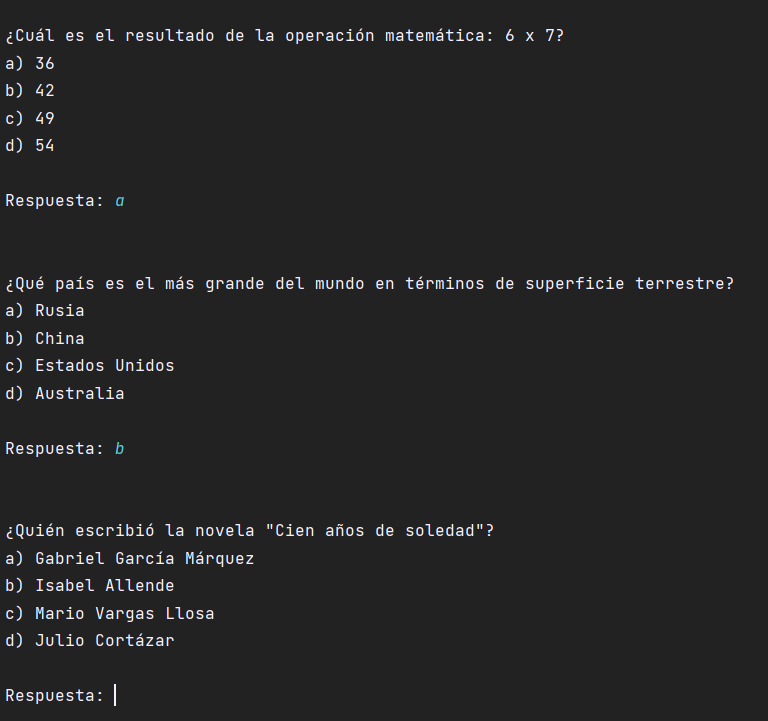
\includegraphics[width=0.7\textwidth,keepaspectratio]{img/Ejemplo1.png}
		%\includesvg{img/automata.svg}
		%\label{img:mot2}
		%\caption{Product backlog.}
	\end{figure}
	\clearpage
	\begin{itemize}	
		\item En este apartado se muestra el resultado obtenido por el usuario:
	\end{itemize}	
	
	\begin{figure}[H]
		\centering
		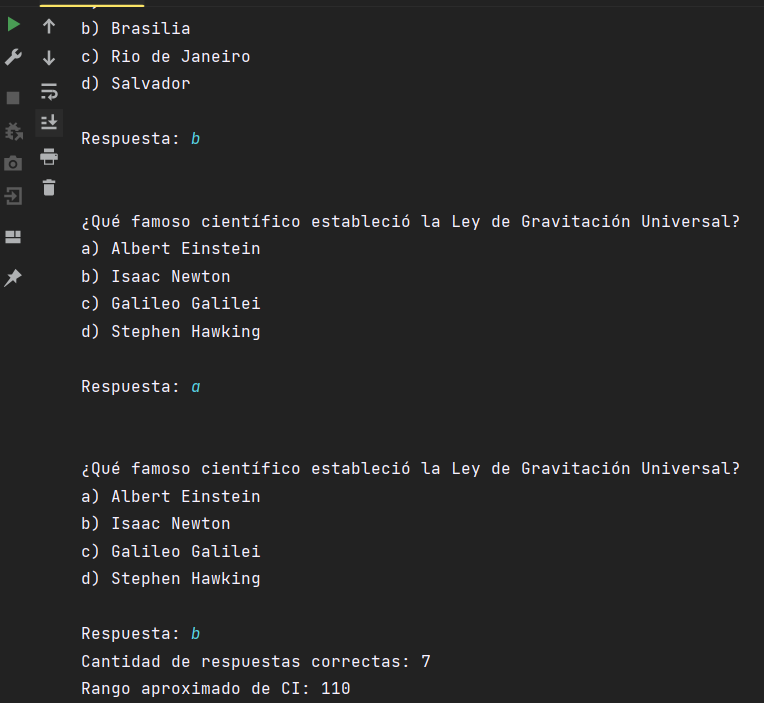
\includegraphics[width=0.7\textwidth,keepaspectratio]{img/Ejemplo2.png}
		%\includesvg{img/automata.svg}
		%\label{img:mot2}
		%\caption{Product backlog.}
	\end{figure}
	\clearpage
	\subsection{Commits del trabajo}
	\begin{itemize}	
		\item Acá estan algunos de los commits mas importantes en este trabajo:
	\end{itemize}	
	
	\begin{figure}[H]
		\centering
		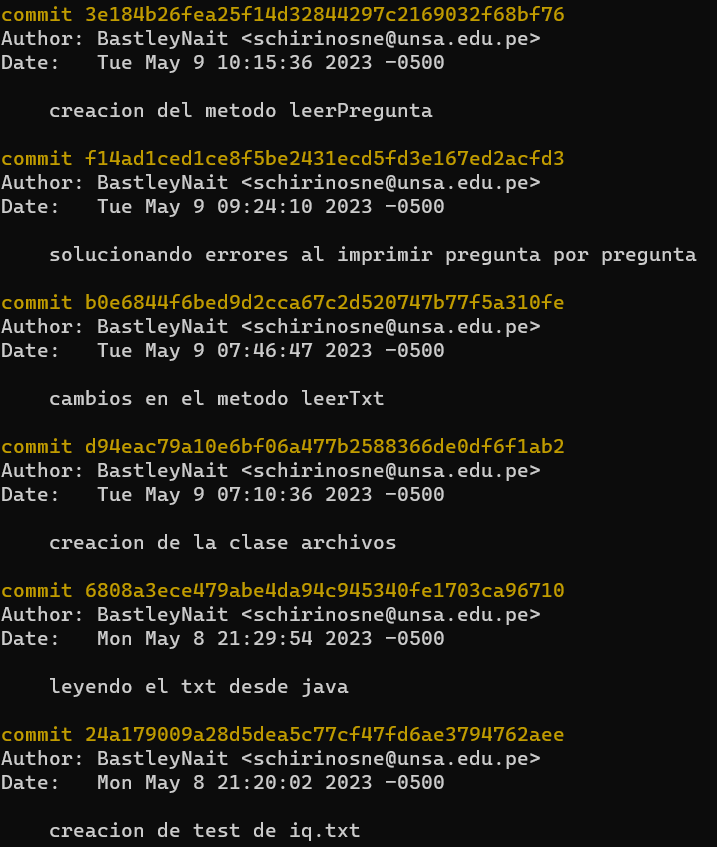
\includegraphics[width=0.5\textwidth,keepaspectratio]{img/Commits.png}
		%\includesvg{img/automata.svg}
		%\label{img:mot2}
		%\caption{Product backlog.}
	\end{figure}


%%%%%%%%%%%%%%%%%%%%%%%%%%%%%%%%%%%%%%%%%%%%%%%%%%%%%%%%%%%%%%%%%%%%%%%%%%%%%%%%%%
	
		
	\subsection{Estructura de laboratorio 01}
	\begin{itemize}	
		\item El contenido que se entrega en este laboratorio es el siguiente:
	\end{itemize}
	
\begin{lstlisting}[style=ascii-tree]
lab01/
|   .gitignore
|   Archivos.java
|   leeme.md
|   Main.java
|   TestdeIQ.txt
|
\---latex
    |   Pweb02_lab04_schirinosne.tex
    |
    +---img
    |       Commits.png
    |       Ejemplo1.png
    |       Ejemplo2.png
    |       logo_abet.png
    |       logo_episunsa.png
    |       logo_unsa.jpg
    |
    \---src
            Archivos.java
            Main.java
            TestdeIQ.txt
\end{lstlisting}    

\section{Pregunta: ¿Por qué Git y GitHub son herramientas importantes para el curso?}
	\begin{itemize}
		\item  Git y GitHub son herramientas esenciales en el desarrollo de software colaborativo y en el control de versiones de proyectos. En el contexto del curso, tienen varias ventajas:
		\item Control de versiones: Git permite realizar un seguimiento detallado de los cambios en el código fuente, lo que facilita la colaboración y permite deshacer o revertir cambios en caso de ser necesario.
		\item Colaboración: GitHub proporciona una plataforma centralizada para compartir y colaborar en proyectos. Los estudiantes pueden trabajar juntos, compartir código, realizar revisiones de código y gestionar tareas de manera eficiente.
		\item Desarrollo de habilidades técnicas: Al utilizar Git y GitHub, los estudiantes adquieren habilidades en el uso de herramientas modernas de desarrollo de software y colaboración, que son altamente valoradas en la industria.
	\end{itemize}	
	\section{Pregunta: ¿Qué conductas éticas deberían promocionarse cuando se usa un Sistema de Control de Versiones?}
	\begin{itemize}
		\item Al utilizar un sistema de control de versiones, es importante promover conductas éticas, tales como:
		\item Respeto a la propiedad intelectual: No utilizar ni compartir código sin la debida autorización o atribución. Respetar las licencias y derechos de autor aplicables.
		\item Evitar la introducción deliberada de código malicioso o de baja calidad. Mantener altos estándares de calidad y asegurarse de que el código sea seguro y eficiente.
		\item Respeto a las contribuciones de otros: Valorar y reconocer el trabajo y las contribuciones de los demás miembros del equipo. Respetar los roles y responsabilidades de cada persona en el proyecto.


	\end{itemize}	
	\section{Pregunta: ¿Qué son los entándares de codificación?}
	\begin{itemize}
		\item  Los estándares de codificación son pautas o reglas establecidas para escribir código de manera consistente y legible. Estos estándares ayudan a mejorar la calidad del código y facilitan su mantenimiento. Algunos aspectos comunes de los estándares de codificación incluyen:
		\item Convención de nomenclatura: Establecer reglas para nombrar variables, funciones y archivos de manera coherente y significativa.
		\item Indentación y espaciado: Definir la forma en que se deben usar los espacios y tabulaciones para mejorar la legibilidad del código.
		\item Comentarios: Fomentar el uso de comentarios claros y concisos para explicar la lógica y el propósito del código.
		\item Definir una estructura lógica y coherente para el código, utilizando bloques, funciones y módulos de manera adecuada.
	\end{itemize}	
\section{\textcolor{red}{Rúbricas}}
	
	\subsection{\textcolor{red}{Entregable Informe}}
	\begin{table}[H]
		\caption{Tipo de Informe}
		\setlength{\tabcolsep}{0.5em} % for the horizontal padding
		{\renewcommand{\arraystretch}{1.5}% for the vertical padding
		\begin{tabular}{|p{3cm}|p{12cm}|}
			\hline
			\multicolumn{2}{|c|}{\textbf{\textcolor{red}{Informe}}}  \\
			\hline 
			\textbf{\textcolor{red}{Latex}} & \textcolor{blue}{El informe está en formato PDF desde Latex,  con un formato limpio (buena presentación) y facil de leer.}   \\ 
			\hline 
			
			
		\end{tabular}
	}
	\end{table}
	\subsection{\textcolor{red}{Rúbrica para el contenido del Informe y demostración}}
	\begin{itemize}			
		\item El alumno debe marcar o dejar en blanco en celdas de la columna \textbf{Checklist} si cumplio con el ítem correspondiente.
		\item Si un alumno supera la fecha de entrega,  su calificación será sobre la nota mínima aprobada, siempre y cuando cumpla con todos lo items.
		\item El alumno debe autocalificarse en la columna \textbf{Estudiante} de acuerdo a la siguiente tabla:
	
		\begin{table}[ht]
			\caption{Niveles de desempeño}
			\begin{center}
			\begin{tabular}{ccccc}
    			\hline
    			 & \multicolumn{4}{c}{Nivel}\\
    			\cline{1-5}
    			\textbf{Puntos} & Insatisfactorio 25\%& En Proceso 50\% & Satisfactorio 75\% & Sobresaliente 100\%\\
    			\textbf{2.0}&0.5&1.0&1.5&2.0\\
    			\textbf{4.0}&1.0&2.0&3.0&4.0\\
    		\hline
			\end{tabular}
		\end{center}
	\end{table}	
	
	\end{itemize}
	
	\begin{table}[H]
		\caption{Rúbrica para contenido del Informe y demostración}
		\setlength{\tabcolsep}{0.5em} % for the horizontal padding
		{\renewcommand{\arraystretch}{1.5}% for the vertical padding
		%\begin{center}
		\begin{tabular}{|p{2.7cm}|p{7cm}|x{1.3cm}|p{1.2cm}|p{1.5cm}|p{1.1cm}|}
			\hline
    		\multicolumn{2}{|c|}{Contenido y demostración} & Puntos & Checklist & Estudiante & Profesor\\
			\hline
			\textbf{1. GitHub} & Hay enlace URL activo del directorio para el  laboratorio hacia su repositorio GitHub con código fuente terminado y fácil de revisar. &2 &X &2 & \\ 
			\hline
			\textbf{2. Commits} &  Hay capturas de pantalla de los commits más importantes con sus explicaciones detalladas. (El profesor puede preguntar para refrendar calificación). &4 & x&2 & \\ 
			\hline 
			\textbf{3. Código fuente} &  Hay porciones de código fuente importantes con numeración y explicaciones detalladas de sus funciones. &2 &X &2 & \\ 
			\hline 
			\textbf{4. Ejecución} & Se incluyen ejecuciones/pruebas del código fuente  explicadas gradualmente. &2 &X &2 & \\ 
			\hline			
			\textbf{5. Pregunta} & Se responde con completitud a la pregunta formulada en la tarea.  (El profesor puede preguntar para refrendar calificación).  &2 &X &2 & \\ 
			\hline	
			\textbf{6. Fechas} & Las fechas de modificación del código fuente estan dentro de los plazos de fecha de entrega establecidos. &2 &X &2 & \\ 
			\hline 
			\textbf{7. Ortografía} & El documento no muestra errores ortográficos. &2 &X &2 & \\ 
			\hline 
			\textbf{8. Madurez} & El Informe muestra de manera general una evolución de la madurez del código fuente,  explicaciones puntuales pero precisas y un acabado impecable.   (El profesor puede preguntar para refrendar calificación).  &4 &x &4 & \\ 
			\hline
			\multicolumn{2}{|c|}{\textbf{Total}} &20 & &18 & \\ 
			\hline
		\end{tabular}
		%\end{center}
		%\label{tab:multicol}
		}
	\end{table}
	
\clearpage		

\section{Referencias}
\begin{itemize}			
	\item \url{https://git-scm.com/book/es/v2}
	\item \url{https://guides.github.com/}
	\item \url{https://www.linuxtrainingacademy.com/nano-emacs-vim/}
	\item \url{h https://cmd.com/blog/vim-or-emacs-the-debate-is-over/}
	\item \url{http://www.viemu.com/vi-vim-cheat-sheet.gif}

\end{itemize}	

	
%\clearpage
%\bibliographystyle{apalike}
%\bibliographystyle{IEEEtranN}
%\bibliography{bibliography}
			
\end{document}